\documentclass[a4paper]{article}
\usepackage[utf8]{inputenc}
\usepackage[english]{babel}
\usepackage{pdfpages, titling}
\usepackage{array, float}
\usepackage{cite, tablefootnote}
\usepackage{graphicx, caption, subfigure,subfig, wrapfig}
\usepackage{listings}
\usepackage{color}
\usepackage{mathtools, braket}
\usepackage{amssymb}
\usepackage[nottoc]{tocbibind} % references in the toc
% \usepackage{subcaption}
\usepackage{textcomp}
\usepackage{minted}
\usepackage[hidelinks]{hyperref}
\graphicspath{{Pictures/}} % Specifies the directory where pictures are stored

\newcommand{\vect}[1]{\boldsymbol{#1}}
\newcommand{\subtitle}[1]{
  \posttitle{
    \par\end{center}
    \begin{center}\large#1\end{center}
    \vskip0.5em}
}
\lstset{frame=tb,
  language=Java,
  aboveskip=3mm,
  belowskip=3mm,
  showstringspaces=false,
  columns=flexible,
  basicstyle={\small\ttfamily},
  numbers=none,
  breaklines=true,
  breakatwhitespace=true,
  tabsize=3
}

\author{Jaro Camphuijsen (6042473) and Rahiel Kasim (10447539)}
\title{Scientific Computing I}
\subtitle{Exploring the SciCoPyth's mind}
\begin{document}
\maketitle

\tableofcontents

\section{Tools}
\textbf{Rahiel}: I've been using Linux for many years now. My favourite programming tool (and favourite software all-round) is GNU Emacs. It is a very advanced text editor. You can better understand Emacs if you think of it as a Lisp virtual machine with many functions for text editing. This means that any editing operation is actually a lisp function, so you can use lisp itself to extend the editor in any way you want. You however don't have to do everything yourself because Emacs has a built-in package manager, with more than 3000 packages available. For newcomers I recommend using \url{www.spacemacs.org}, a community maintained Emacs configuration with a focus on Vim emulation. 

Another tool that is more easily adopted in someone's existing workflow is z (\url{www.github.com/rupa/z/}). It tracks which directories you use most often so you can more easily jump to them. For example, if I type \texttt{z bio} it cd's my shell to \texttt{\~{}/Dropbox/univ/Computational Biology}, and \texttt{z chrom} brings me to \texttt{\~{}/Code/archiveror/chromium}.

I am going to become a better programmer simply by programming more and by studying more ways how people program to solve problems.
\\ \\
\noindent
\textbf{Jaro}: I have used Linux in the past on some other machines however after two months in my Masters Computational Science of using Windows on my own laptop, Rahiel convinced me to switch to Linux. It has made my life easier from the very beginning, and with the text editor Emacs almost anything is possible. It has a steeper learning curve then other text editors, but once you know the basic key combination the more complex operations become very easy and less time consuming. \\
For sharing our code Rahiel and I like to use GitHub~\cite{sunsistemoGH}, it keeps track of changes and you can find back older versions at any time. Another nice function of GitHub is adding so called "issues" to your repository, this you can keep track of bugs and it also gives you a to do list towards the end of your project. \\
For reporting we like to use \LaTeX \ because of its easy and clean layout generation, it automatically places figures and tables at good locations and keeps track of the reference numbers. \LaTeX \  files can also be shared on GitHub, however better tools exist like \url{www.sharelatex.com} and \url{www.overleaf.com}, where you can edit your online \LaTeX \ files interactively. 

\section{Vibrating String}
The time evolution of a vibrating string is given by the partial differential equation \ref{eq:wave1D}

\begin{equation}
\frac{\partial ^2 \Psi}{\partial  t^2} = c^2 \frac{\partial ^2 \Psi}{\partial dx^2} 
\label{eq:wave1D}
\end{equation}

To get a unique solution for $\Psi (x,t)$ we have to declare boundary and initial conditions.

% \begin{subequations}
% \begin{align}
% \Psi (x, t_1) = f_1(x)\\
% \Psi '(x,t_2) = f_2(x)\\
% \Psi (x_1, t) = g_1(t)\\
% \Psi (x_2,t) = g_2(t)
% \label{eq:wave1Dinit}
% \end{align}
% \end{subequations}

\noindent\begin{minipage}{.5\linewidth}
\begin{equation*}
\Psi (x, 0) = f(x)
\end{equation*}
\end{minipage}
\begin{minipage}{.5\linewidth}
\begin{equation*}
\Psi (0, t) = 0
\end{equation*}
\end{minipage}\\
\begin{minipage}{.5\linewidth}
\begin{equation*}
\Psi '(x,0) = 0
\end{equation*}
\end{minipage}
\begin{minipage}{.5\linewidth}
\begin{equation*}
\Psi (L,t) = 0
\end{equation*}
\end{minipage}
\label{eq:wave1Dinit}

For the initial position of the string we use three different cases:
\begin{subequations}
\begin{align}
f(x) &= \sin (2 \pi x)\\  
\label{eq:init2} f(x) &= \sin (5 \pi x)\\
f(x) &= \sin (5 \pi x) \qquad \text{if } \frac{1}{5} \le x \le \frac{2}{5} \text{, else } \Psi = 0
\end{align}
\end{subequations}

Only in a few cases can this PDE be solved analytically, hence we would like to construct a numerical model. To do this we discretize the continuous problem. For time step $k$ and spatial step $i$ we can write for the partial second derivatives of $\Psi$:

\begin{subequations}
\begin{align}
\frac{\partial ^2 \Psi}{\partial  x^2} &= \frac{u^{k}_{i+1} - 2 u^{k}_{i} + u^{k}_{i-1}}{\Delta x^2}\\
\frac{\partial ^2 \Psi}{\partial  t^2} &= \frac{u^{k+1}_{i} - 2 u^{k}_{i} + u^{k-1}_{i}}{\Delta t^2}
\end{align}
\end{subequations}

Now we can solve the discrete (1D) wave equation for $u^{k+1}_{i}$ so we can compute the new value of each spatial bin $i$ from the current and previous time steps and its surrounding bins \cite{sciComp}:

\begin{equation}
u^{k+1}_{i} = 2 u^{k}_{i} - u^{k-1}_{i} + c \left ( \frac{\Delta t}{\Delta x} \right ) ^2 \left ( u^{k}_{i+1} - 2 u^{k}_{i} + u^{k}_{i-1} \right ), \qquad i = 1, ... , n
\end{equation}

We've implemented this scheme and in figure \ref{fig:wave} we see solutions to the wave equation with the initial conditions of eq. \ref{eq:init2}. We also have animations that better elucidate the time evolution and the inevitable numerical instability.

\begin{figure}
\center{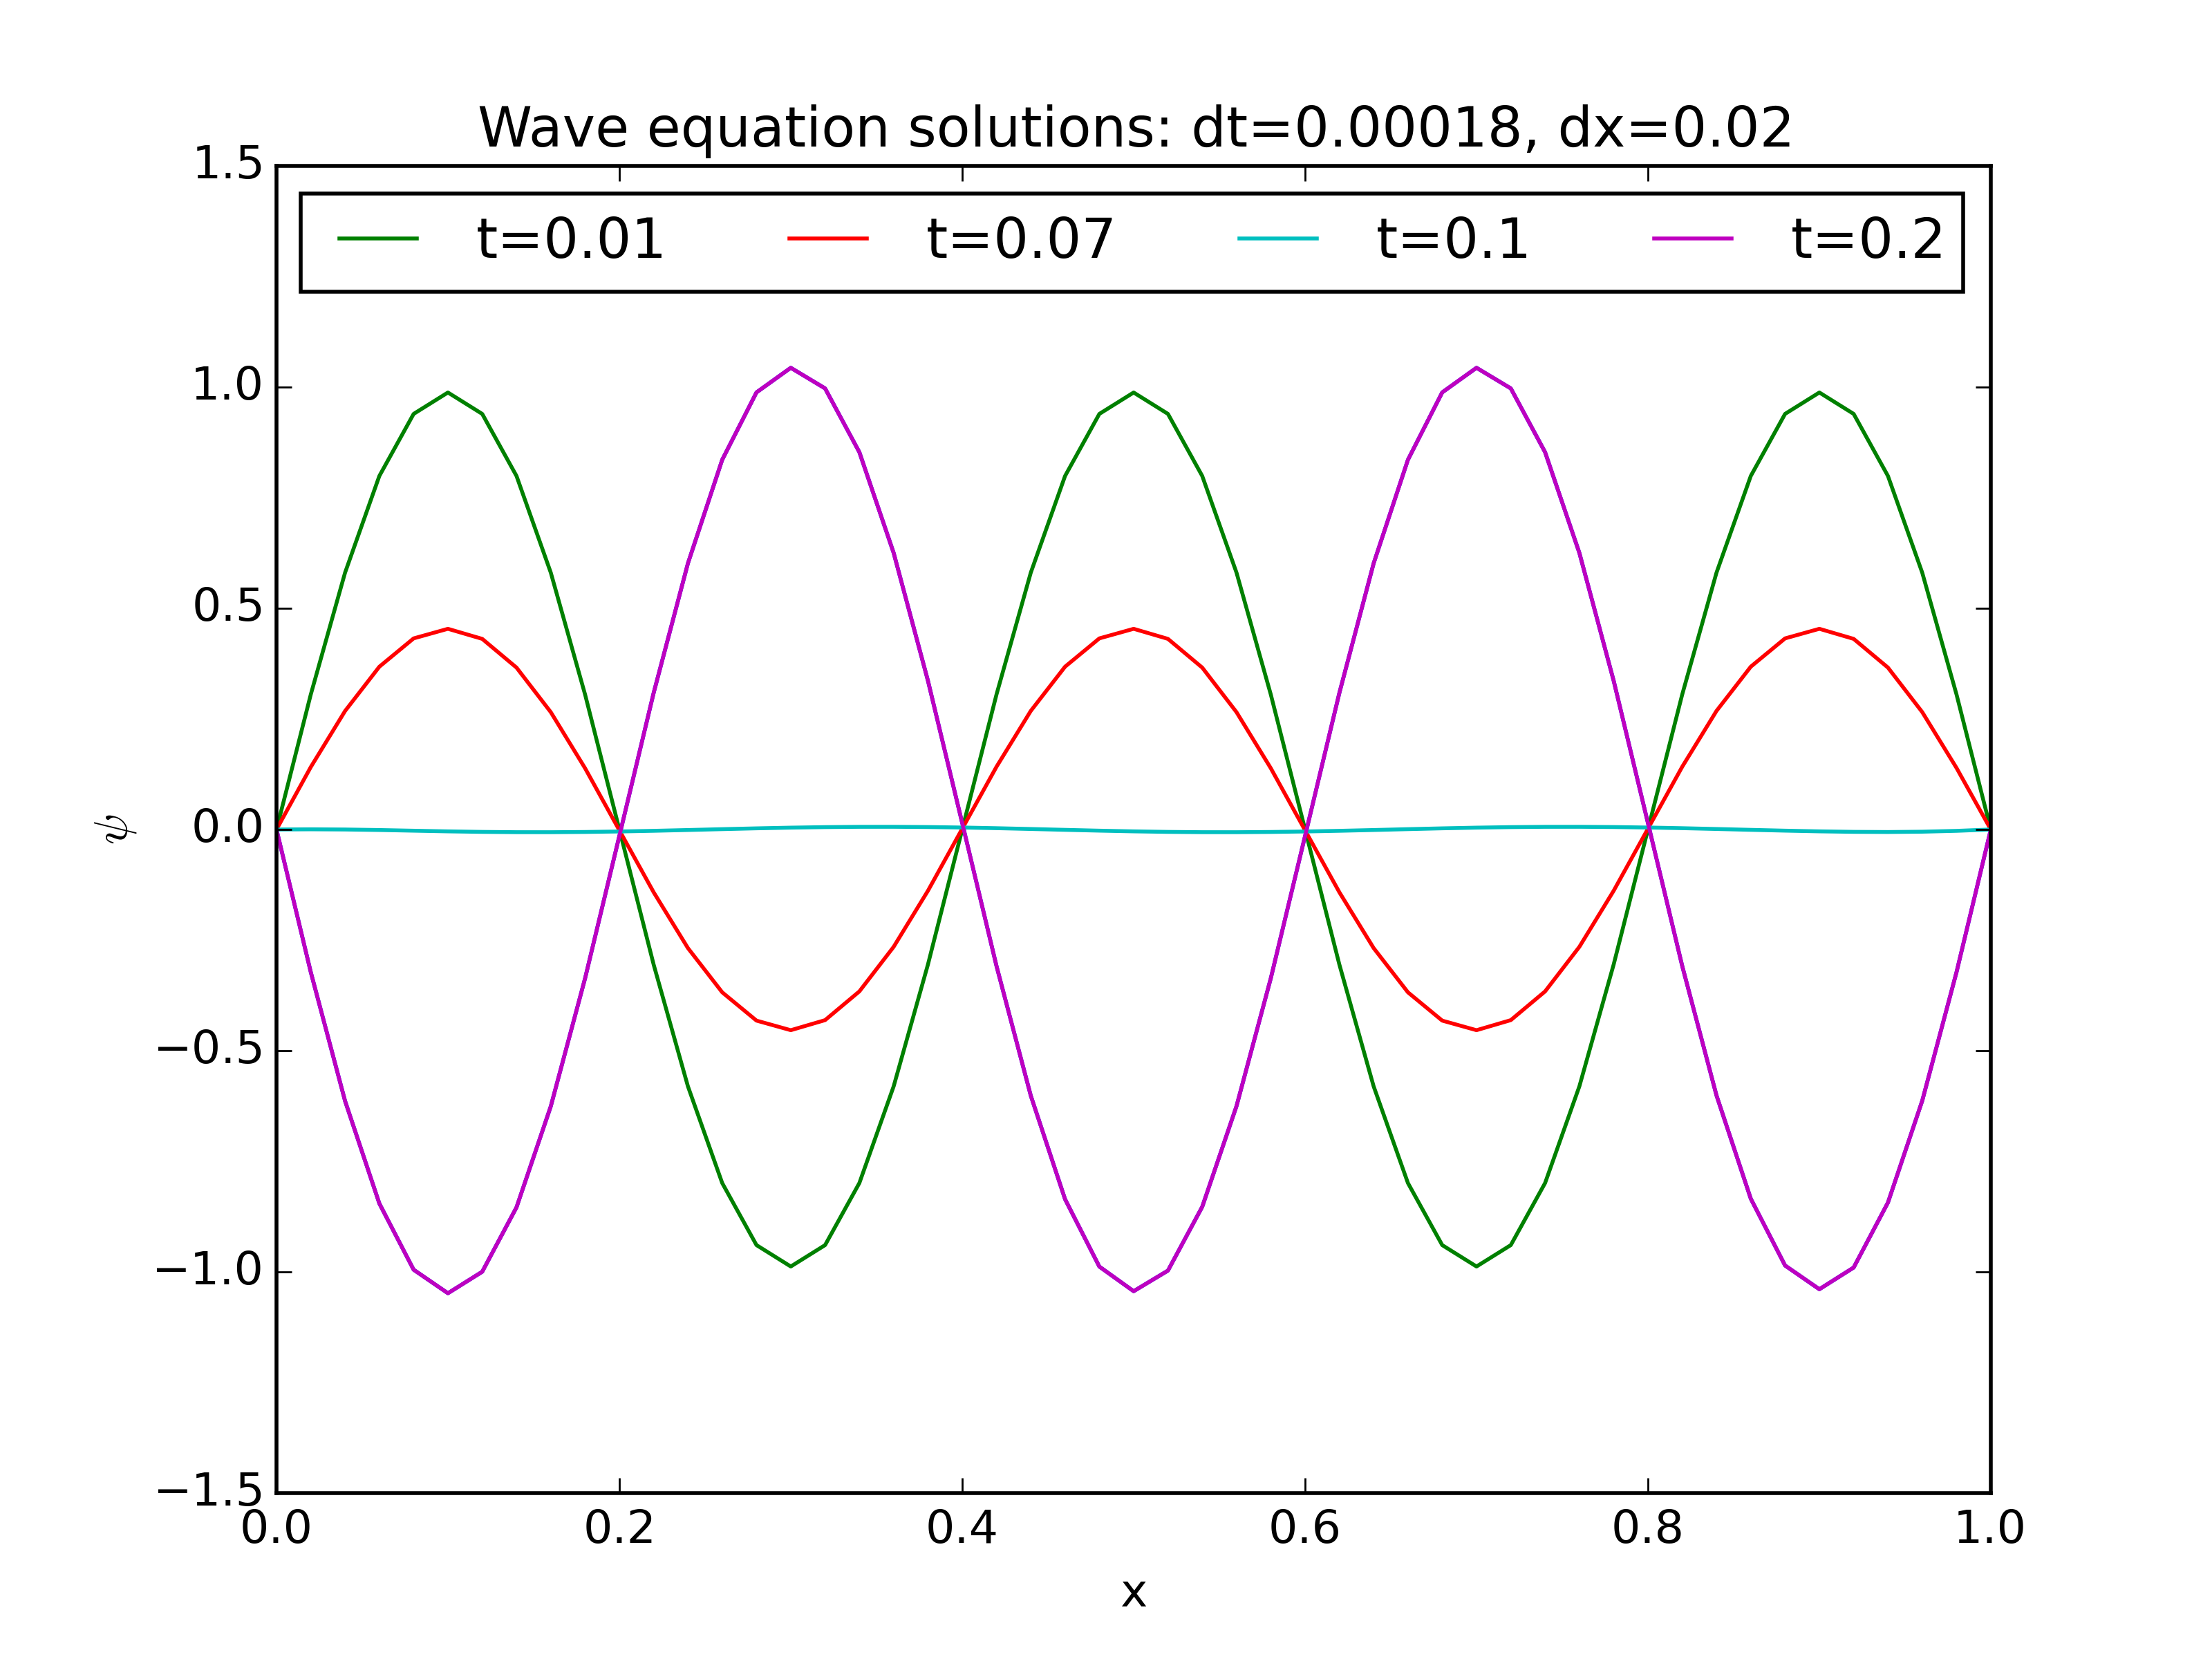
\includegraphics[height=8cm]{wave_eq}}
\caption{Solutions to the wave equation calculated with the finite difference method described in the text.}
\label{fig:wave}
\end{figure}

% Same in code:
% \begin{minted}{python}
% for i in range(1, N-1)
%     u2[i] = 2u1[i] - u0[i] + c (dt/dx)^2 (u1[i+1] - 2 u1[i] + u1[i-1])
% \end{minted}
% \label{code:wave1D}



\section{The Time Dependent Diffusion Equation}

\begin{equation}
c^{k+1}_{i,j} = c^{k}_{i,j} +  \frac{\Delta t}{\Delta x^2} \left ( u^{k}_{i+1,j} +u^{k}_{i-1,j} + u^{k}_{i,j+1} + u^{k}_{i,j+1}
 \right ), \qquad i = 1, ... , n
\end{equation}

At the boundaries of the x domain from we use the following function values to make periodic boundary conditions: 

\begin{subequations}
\begin{align}
u^{k}_{N+1,j} = u^{k}_{0,j}\\
u^{k}_{-1,j} = u^{k}_{N,j} 
\end{align}
\end{subequations}

for the boundaries of the y domain we lock the values of $u^{k}_{i,0}$ and $u^{k}_{i,N}$ to respectively 1 and 0. We then let the simulation only generate values in the y domain \{1, N-1 \}.

The simulation was done with N=30 spatial bins in both the x and y direction, the value of the time step was determined by the stability constraint:

\begin{equation}
    \Delta t = 0.9 \frac{\Delta x^2}{4 D}
\end{equation}

For this specific configuration we can compute the analytic solution:

\begin{equation}
    c(x,t) = 1 - \sum\limits_{i=1}^{\inf} \left [ \text{erfc} \left (\frac{1 - x + 2i}{2 \sqrt{D t}} \right ) - \text{erfc} \left (\frac{1 + x + 2i}{2 \sqrt{D t}} \right ) \right]
\end{equation}

And so we can compare the analytic solution with our model. The result for at different points in time can be seen in figure \ref{fig:1Ddiffusion} where we dispose of the x dimension. This can be done without loss of information since $u$ is constant along the x dimension, due to the configuration of this simulation. The full two dimensional outcome can be found in figure \ref{fig:2Ddiffusion} where heatmaps are drawn for the same points in time as in figure \ref{fig:1Ddiffusion}. In addition an animated plot was made which can be viewed by running the code. 

\begin{figure}
\center{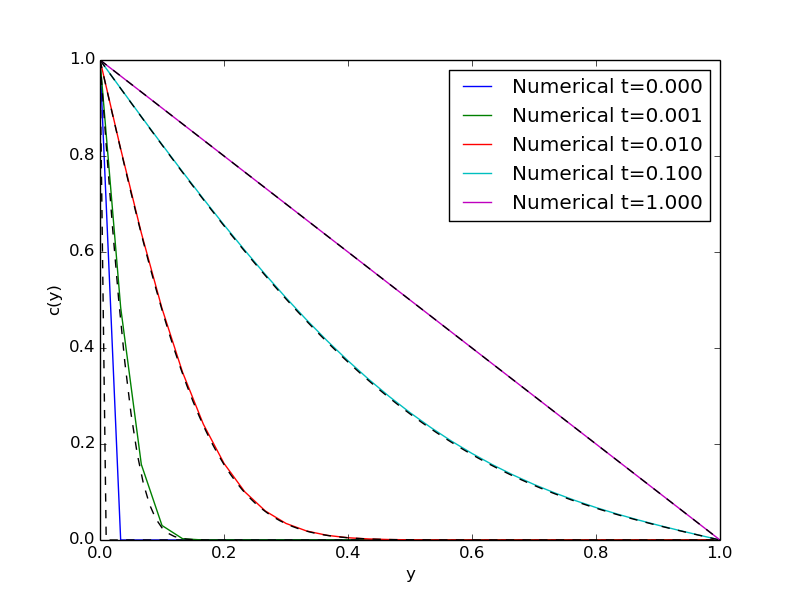
\includegraphics[height=8cm]{diffusion1D.png}}
\caption{Comparison of the analytic solution (dashed line) and the numerical model at several points in time for the time dependent diffusion equation }
\label{fig:1Ddiffusion}
\end{figure}

\begin{figure}[h]
\centering
\subfloat[]{
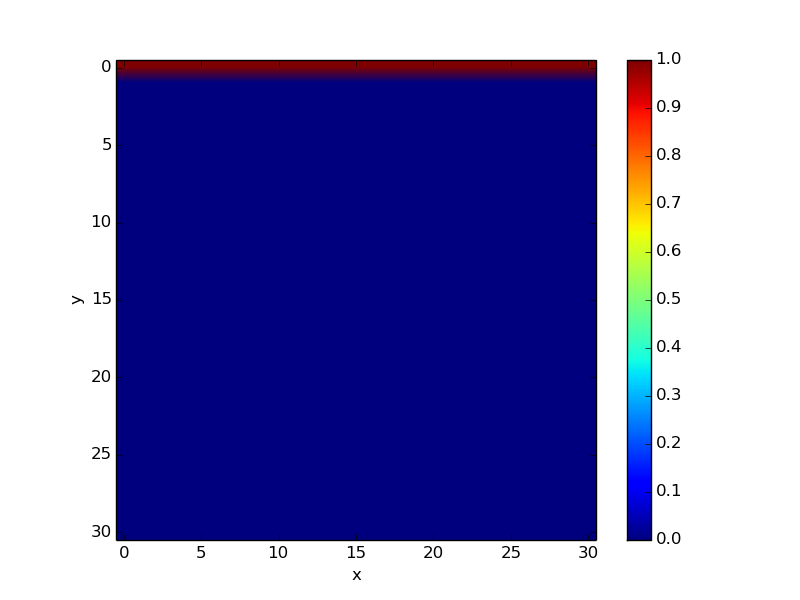
\includegraphics[width=0.4\textwidth]{diffusion_1.png}
}
\subfloat[]{
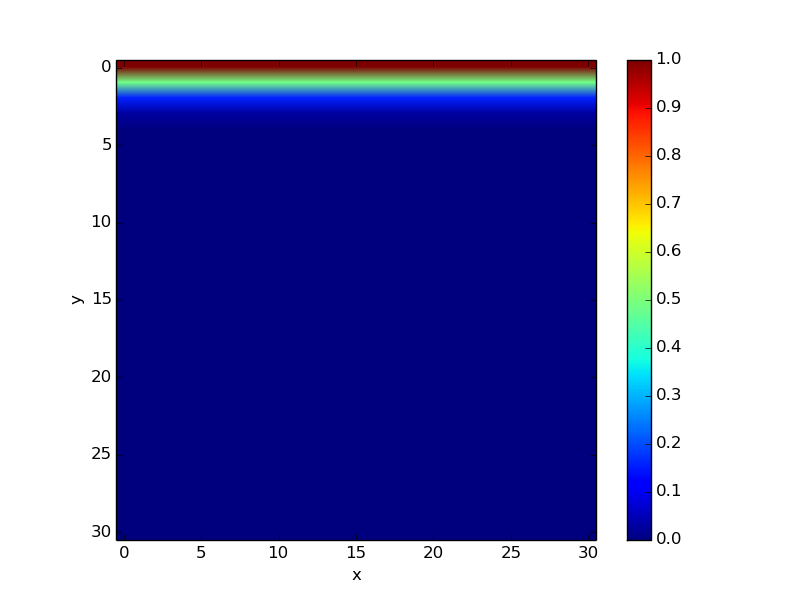
\includegraphics[width=0.4\textwidth]{diffusion_2.png}
}\\
\subfloat[]{
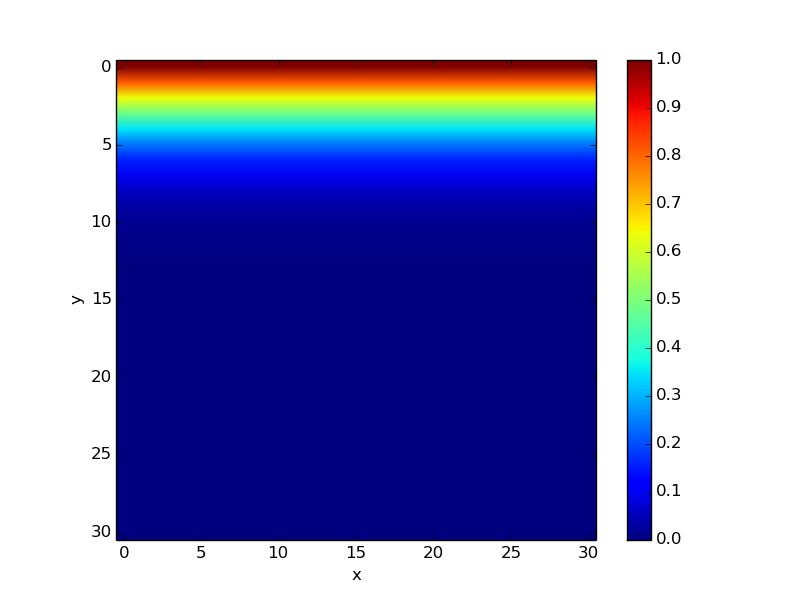
\includegraphics[width=0.4\textwidth]{diffusion_3.png}
}
\subfloat[]{
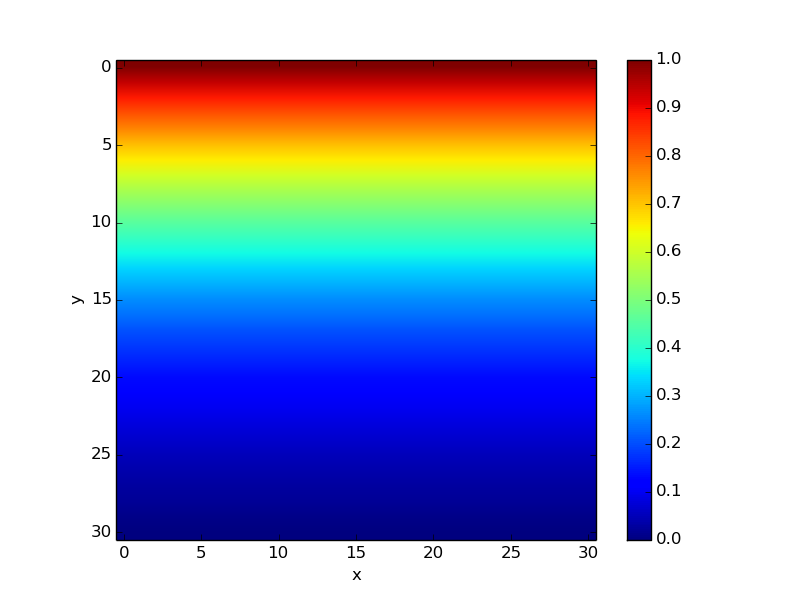
\includegraphics[width=0.4\textwidth]{diffusion_4.png}
}\\
\subfloat[]{
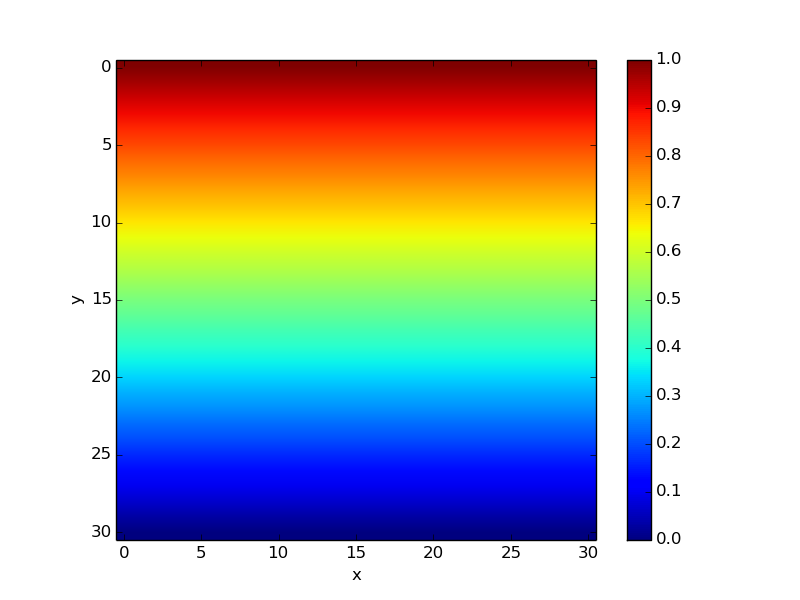
\includegraphics[width=0.4\textwidth]{diffusion_5.png}
}
\caption{Several stages in the time dependent diffusion simulation in a 2 dimensional heatmap, the plots correspond to respectively t = [0, 0.001, 0.01, 0.1, 1]}
\label{fig:2Ddiffusion}
\end{figure}


\section{The Time Independent Diffusion Equation}
We've implemented the Jacobi iteration, Gauss-Seidel method and SOR with $N=50$ and a tolerance of $\epsilon = 10^{-5}$. In figure \ref{fig:time_ind} we compare the results of the three methods with the analytic solution. We see that they all come very close to the analytic solution: the result of SOR is superimposed on the analytic solution ($\lim_{t \to \infty} c(y, t)=-y$), while the Gauss-Seidel is further down and the Jacobi iteration is still below that. The nice thing is that this is also the same order for efficiency of the methods, SOR is both the most efficient (least amount of iterations) and the most accurate (closest to the analytic solution).

\begin{figure}
\center{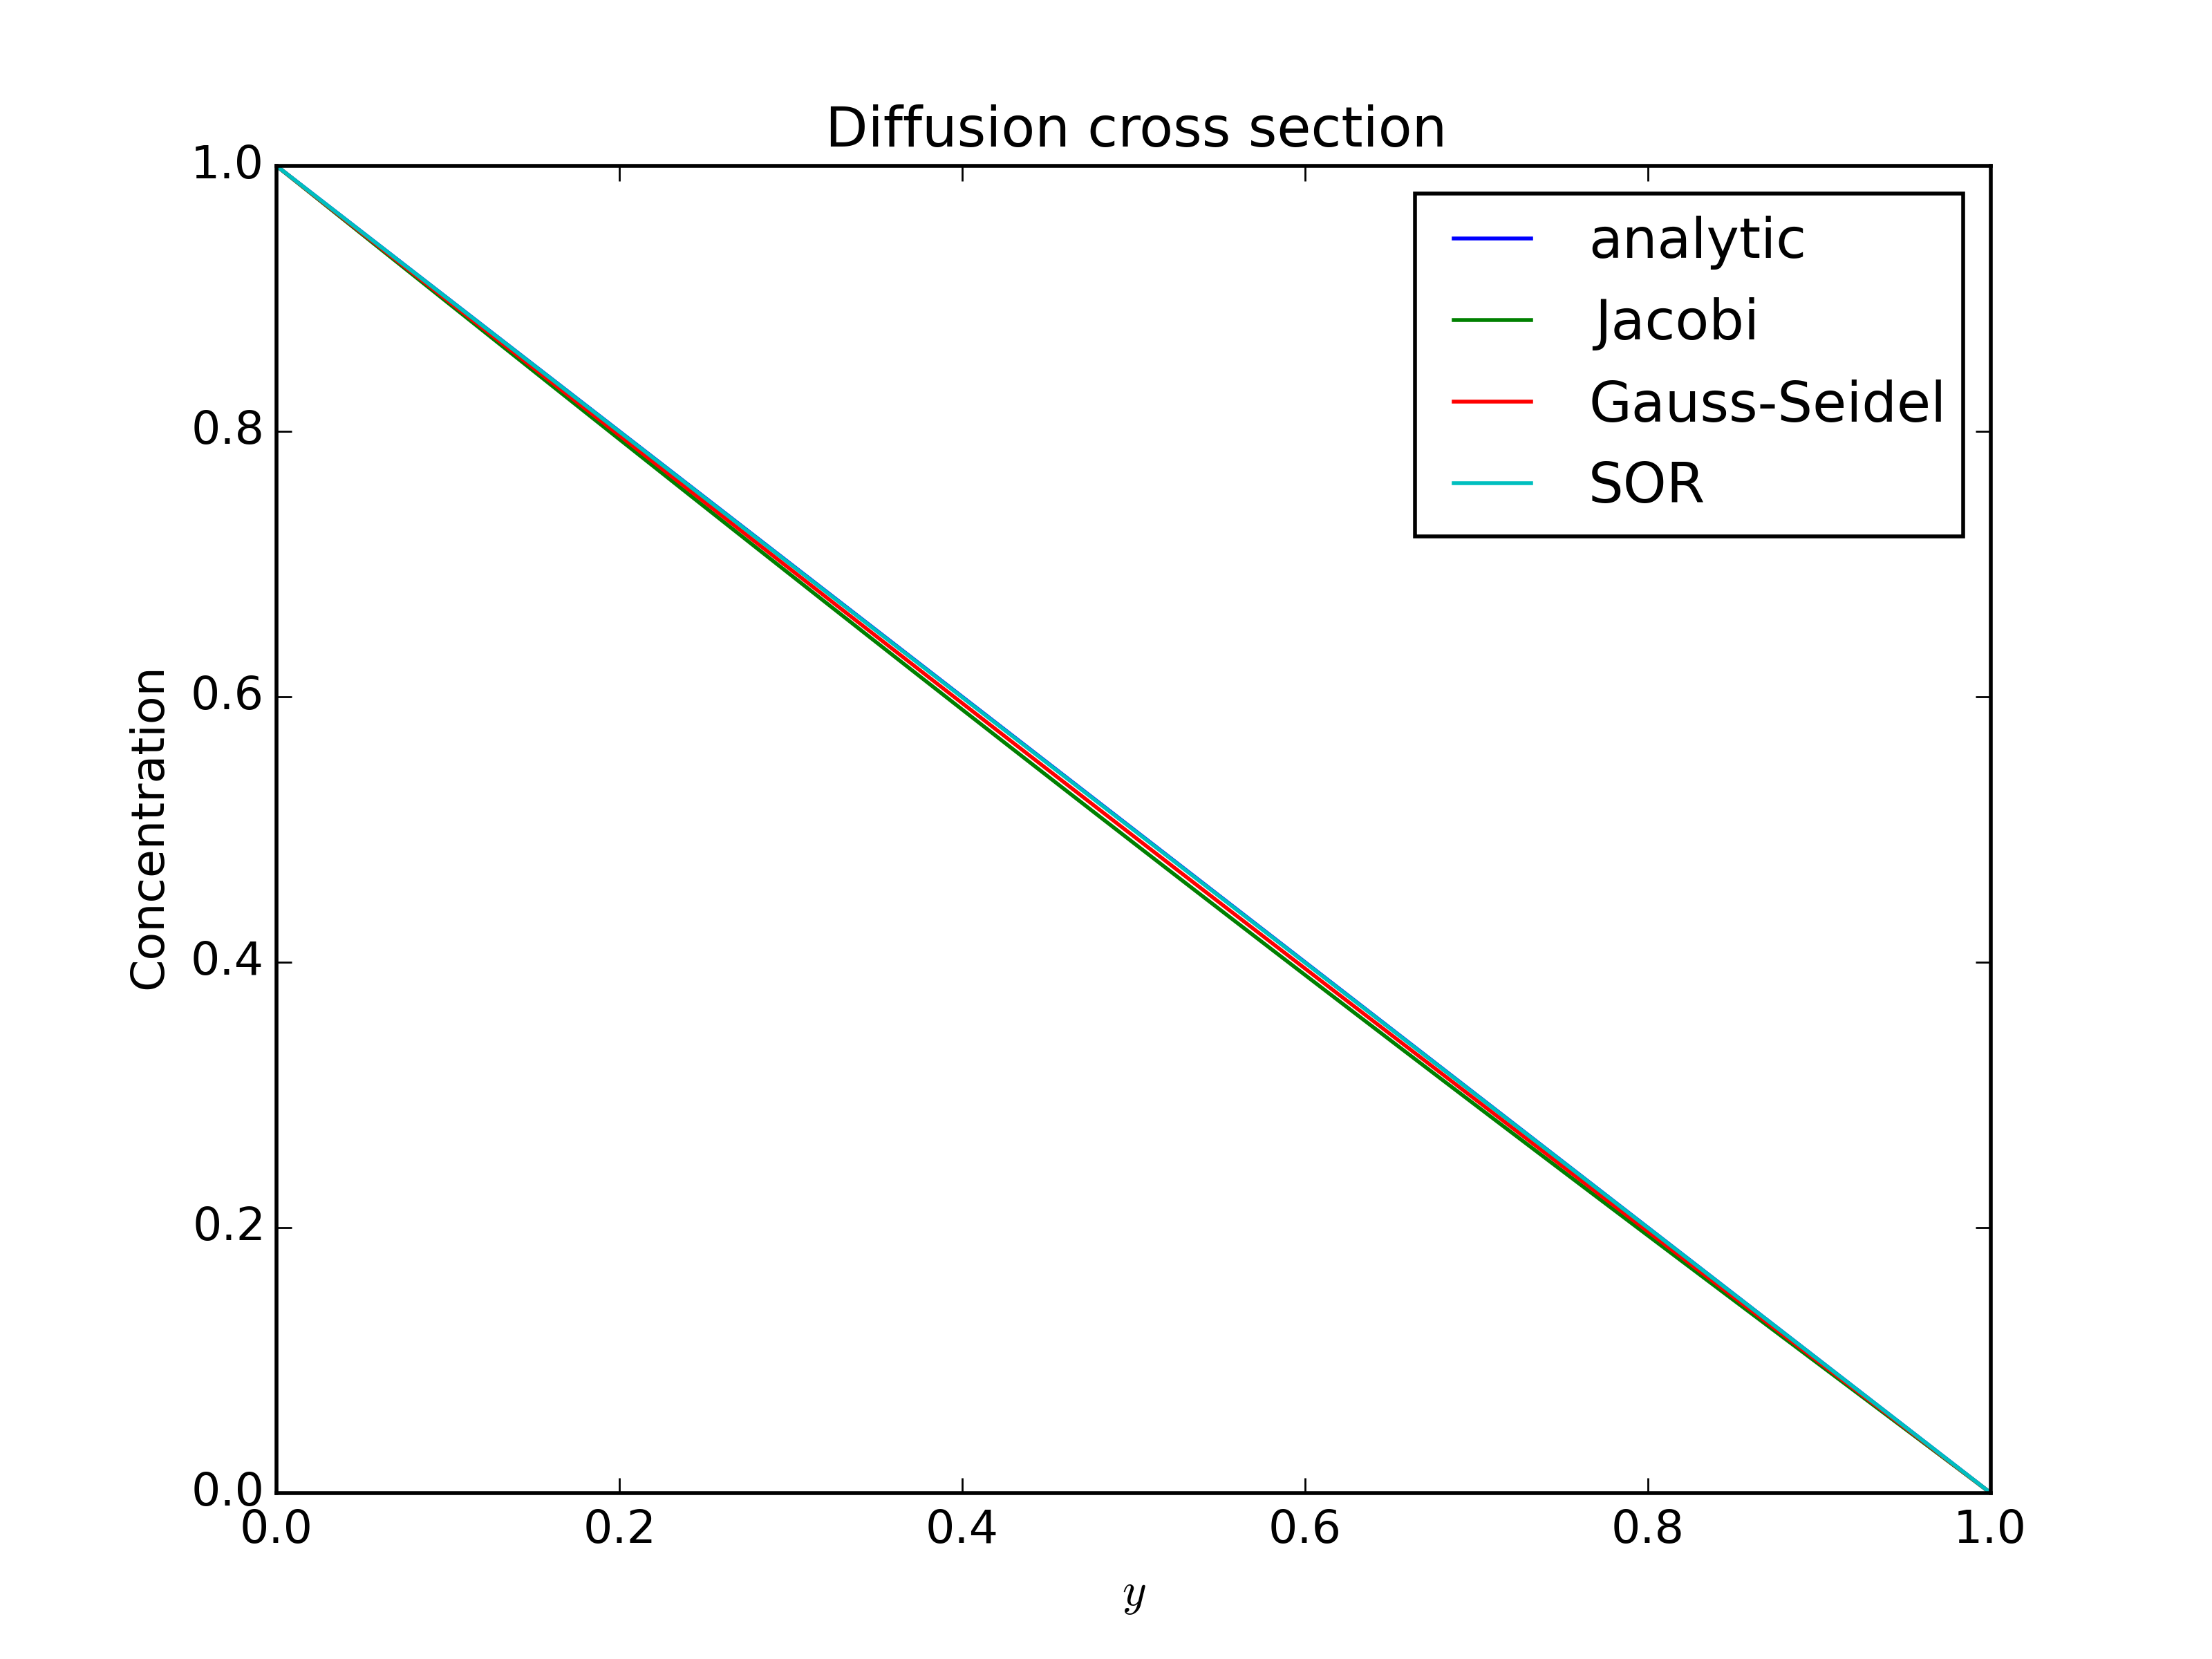
\includegraphics[height=8cm]{time_ind}}
\caption{A cross section of the solution of the time independent diffusion equation for different methods..}
\label{fig:time_ind}
\end{figure}

We can further investigate the efficiency of the methods we've implemented by looking at the convergence measure $\delta$ versus the number of iterations $k$. In figure \ref{fig:conv} we see this relation for the three methods, we again see that the SOR method is the most efficient as it converges at the lowest number of iterations.

\begin{figure}
\center{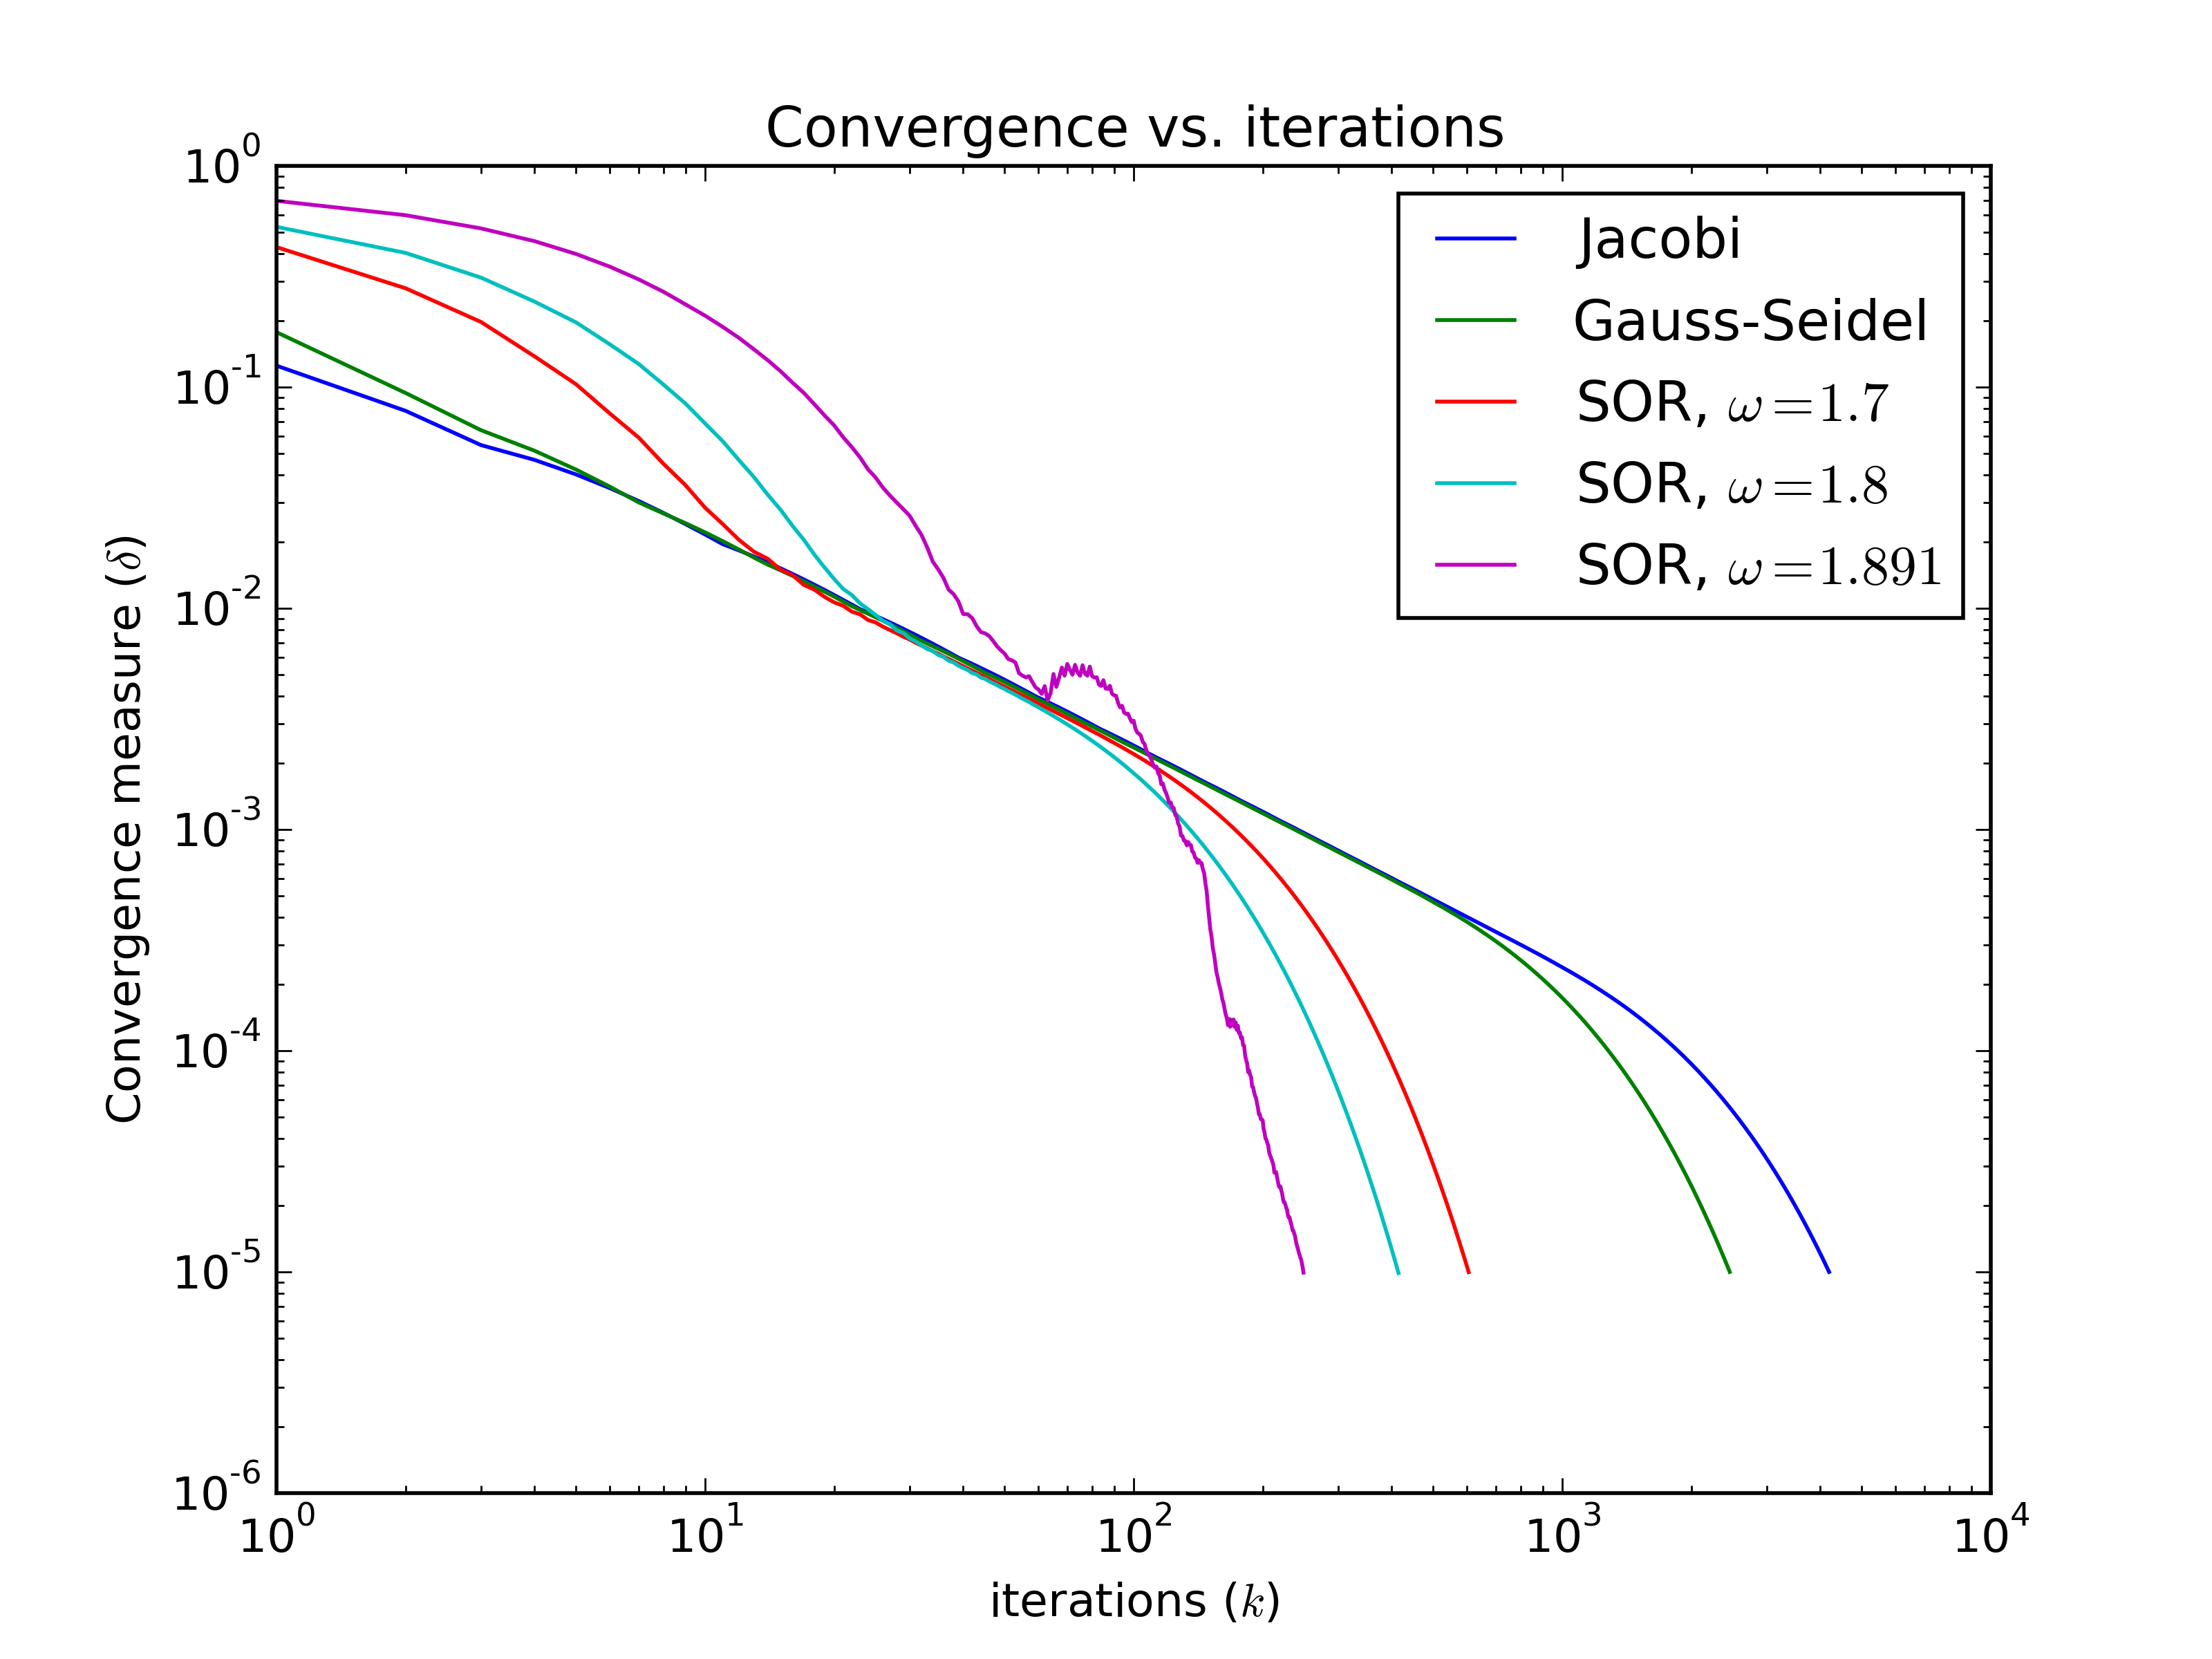
\includegraphics[height=8cm]{time_ind_conv}}
\caption{The convergence measure vs. the number of iterations for the methods solving the time independent diffusion equation. We see that the SOR method converges with the least amount of iterations.}
\label{fig:conv}
\end{figure}

We can find the optimal $\omega$ for the SOR method by doing the SOR computation with different values for $\omega$ between the specified range while looking for the $\omega$ that needs the least amount of iterations. One can find $\omega$ naively by trying all values, or by doing a (binary) search over the range. We found as optimal $\omega = 1.891$. We can also look at the optimal $\omega$ for different values of $N$, using the same method we found that smaller values of $N$ have a smaller optimal $\omega$ (for $N=40$ we found $\omega=1.87$) and for larger $N$ we also find larger $\omega$ (for $N=60$ we found $\omega=1.91$).

We put a 10 x 10 square in the middle of the domain and find that the convergence is faster, it took 204 iterations and without an object it takes 250 iterations. We find a slower convergence of 224 iterations if we put two 5 x 10 rectangles in the domain. Using the same method to find the optimal $\omega$ we find with the 10 x 10 square the optimum $\omega=1.87$ with 159 iterations, so adding an object slightly lowered the optimal $\omega$. For the two 5 x 10 rectangles we find an optimum of $\omega=1.89$ with 222 iterations, so here the object very slightly lowered the optimal.

For these two examples we found that adding objects lowered the iterations and may also lower the optimal $\omega$ value.

\bibliography{references}
\bibliographystyle{unsrt}

\end{document}
